\chapter{Conceitos básicos}
%Basic cloud definitions
Este capítulo introduz as definições e os conceitos básicos quando se trata de Cloud Computing.

\section{Definição de Cloud Computing}
	Computação em Nuvem (do Inglês \textit{Cloud Computing}) é segundo a NIST (\textit{National Institute of Standards and Technology}) um modelo para prover um acesso de rede a um grupo compartilhado (\textit{shared pool}) de recursos computacionais (recursos como capacidade de rede, servidores, armazenamento, aplicações e serviços) de forma ubíqua, prática e sob demanda.

	Tal acesso deve ser rapidamente provisionado e lançado com o mínimo de gerenciamento e interação com o provedor de serviços por parte da aplicação.

	O modelo de computação em nuvem deve possuir algumas características básicas, que estão descritas na secção seguinte.

\section{Características básicas de Cloud Computing}
	A NIST define 5 características essenciais do modelo de Cloud Computing:
	\begin{itemize}
		\item
			Serviço sobre demanda: Um consumidor pode provisionar unilateralmente capacidades computacionais, como tempo de servidor e armazenamento de rede, conforme for necessário, sem qualquer interação humana com o provedor de serviço;
		\item
			Agrupamento de recursos: Os recursos de computação do provedor são agrupados para atender a vários consumidores usando um modelo "multi inquilino", com diferentes recursos físicos e virtuais dinamicamente
			atribuídos e reatribuídos de acordo com a demanda do consumidor. Existe uma sensação de independência de localização pois o cliente geralmente não tem controle ou conhecimento sobre a localização exata dos recursos fornecidos, mas pode ser capaz de especificar a localização em um nível
			abstração (por exemplo, país, estado ou datacenter). Exemplos de recursos incluem armazenamento, processamento, memória e largura de banda de rede.
		\item
			Amplo acesso à rede: Os recursos estão disponíveis na rede e são acessados por meio de mecanismos que promovam o uso por plataformas heterogêneas por clientes em diversos dispositivos (por exemplo, telefones celulares, tablets, laptops e estações de trabalho). Esta característica promove o conceito de computação ubíqua, isto é, em toda parte, onipresente.
		\item
			Elasticidade rápida: Os recursos podem ser provisionados e liberados elasticamente, em alguns casos automaticamente, proporcionando uma escalabilidade crescente ou descrescente conforme a demanda. Os recursos disponíveis normalmente aparentam ser ilimitados para o consumidor, podendo ser requisitidados em qualquer quantidade e a qualquer momento.
		\item
			Serviço mensurável: Os sistemas em nuvem controlam e otimizam automaticamente o uso de recursos, aproveitando-se de uma capacidade de medição em um nível de abstração apropriado ao tipo de serviço (por exemplo, armazenamento, processamento, largura de banda e contas de usuário ativas). O uso de recursos pode ser monitorado, controlado e reportado, gerando transparência tanto para o fornecedor e consumidor do serviço utilizado.
	\end{itemize}


\chapter{Modelos para Cloud Computing}
	Este capítulo introduz brevemente os modelos de serviço de cloud computing que podem ser adotados por um provedor e os modelos de \textit{deployment}, nas secções seguintes.

\section{Modelos de serviços}
	A teoria por trás dos serviços de computação em nuvem abrange três elementos principais: software, plataforma e infraestrutura. Temos os seguintes modelos de serviço:

	\begin{itemize}
		\item
			\textbf{SaaS, Software as a Service} ("Software como um serviço") 

			Neste modelo é oferecido ao consumidor o uso de aplicações de um provedor que rodam sobre uma infraestrutura em nuvem. Estas aplicações são acessíveis a partir de vários dispositivos clientes por meio de uma interface simples, como um navegador da web, ou uma interface de por meio de um programa (mobile ou desktop). 

			O consumidor não gerencia ou controla a infraestrutura de nuvem por trás da aplicação, incluindo rede, servidores, sistemas operacionais, armazenamento ou capacidade da aplicação individual. São disponibilizadas apenas configurações do aplicativo específicas para aquele usuário individual.

			Alguns exemplos de SaaS são serviços de \textit{webmail}, \textit{streaming} de vídeos, conversão de arquivos e trabalho colaborativo com arquivos. Este modelo não será mais detalhado neste trabalho.

		\item
			\textbf{PaaS, Platform as a Service} ("Plataforma como um serviço") 

			A capacidade fornecida ao consumidor é de implantar na nuvem aplicações criadas por meio de linguagens de programação, bibliotecas, serviços e ferramentas suportadas pelo provedor. Tais aplicações podem ser criadas pelo próprio consumidor, ou consumidas por este.

			Assim como no modelo de SaaS, o consumidor geralmente não gerencia ou têm controle sobre a infraestrutura de nuvem por trás, incluindo rede, servidores, sistemas operacionais, ou armazenamento. Porém o consumidor as tem controle sobre os aplicativos implantados e possivelmente sobre definições de configuração para o ambiente de hospedagem do aplicativo.

			Como exemplos de provedores no mercado temos \textit{IBM Bluemix}, \textit{Heroku}, e \textit{Windows Azure Cloud}.
		\item
			\textbf{IaaS, Infrastructure as a Service} ("Infraestrutura como um serviço") 

			A capacidade oferecida ao consumidor é provisionar processamento, armazenamento, redes e outros recursos fundamentais de computação onde o consumidor é capaz de implantar e executar software arbitrário, incluindo-se sistemas e aplicações. O consumidor não gerencia nem controla a infraestrutura de nuvem por trás, mas tem controle sobre sistemas operacionais, armazenamento e aplicativos implantados. Possivelmente possui também um controle limitado de componentes de rede (por exemplo, firewalls de host). Geralmente acompanha serviços de máquinas virtualizadas.

			Alguns exemplos de provedores no mercado são \textit{Amazon Web Services}, \textit{Microsoft Azure}, \textit{Google Cloud} e \textit{VMware Cloud on AWS}. 
	\end{itemize}

\section{Modelos de implantação}
	Os modelos de implantação (\textit{deployment models}) a seguir delimitam as formas possíveis de tarifação dos serviços, as possíveis localizações da infraestrutura física e o público de escopo. São eles:

	\begin{itemize}
		\item
			\textbf{Nuvem privada}: A infraestrutura de nuvem é disponibilizada para uso exclusivo por uma única organização, compreendendo vários consumidores (\textit{business units}). Pode ser propriedade e gerenciada pela própria organização, um terceiro ou alguma combinação de ambos, e pode existir dentro ou fora das instalações da organização.
		\item
			\textbf{Nuvem comunitária}: A infraestrutura em nuvem é de uso exclusivo por uma comunidade de consumidores de organizações que compartilham mesmos interesses (por exemplo, missão, requisitos de segurança, políticas e considerações de conformidade). Pode ser de propriedade e administrada por uma ou mais organizações da comunidade, um terceiro, ou alguma combinação de ambos, e pode existir dentro ou fora das instalações.
		\item
			\textbf{Nuvem pública}: A infraestrutura de nuvem é para o uso aberto pelo público em geral. Pode ser propriedade ou gerenciada por uma organização comercial, acadêmica ou governamental, ou alguma combinação destes. Existe dentro das instalações do provedor de nuvem.
		\item
			\textbf{Nuvem híbrida}: A infraestrutura de nuvem é uma composição de duas ou mais infraestruturas de nuvens distintas (privadas, comunitárias ou públicas) que permanecem como entidades únicas, mas unidas por tecnologia padronizada ou proprietária permitindo portabilidade de dados e aplicações (por exemplo, \textit{cloud bursting} para balanceamento de carga entre nuvens).
	\end{itemize}


\chapter{Arquitetura}
	Este capítulo apresenta uma arquitetura de referência para cloud computing na primeira secção. Na secção final apresenta boas práticas e métodos para arquitetar uma aplicação que deve ser colocada em um ambiente de nuvem.

\section{Arquitetura de referência}
	O objetivo da arquitetura de referência apresentada a seguir é de providenciar uma taxonomia simples e sem ambiguidade para os três modelos de serviço:
	\begin{itemize}
		\item
			Software as a Service (SaaS)
		\item
			Platform as a Service (PaaS)
		\item
			Infrastructure as a Service (IaaS)
	\end{itemize}

	Tal arquitetura deve disponibilizar uma visão unificada das cinco características essenciais da NIST:
	\begin{itemize}
		\item
			Serviço sobre demanda
		\item
			Amplo acesso à rede
		\item
			Agrupamento de recursos
		\item
			Elasticidade rápida (escalabilidade)
		\item
			Serviço mensurável
	\end{itemize}

	Após pesquisar informações disponibilizadas por provedores, instituições de pesquisa e de consultoria na área achamos interessante a seguinte arquitetura de referência:

	\begin{figure}[h!]
  	\centering
  	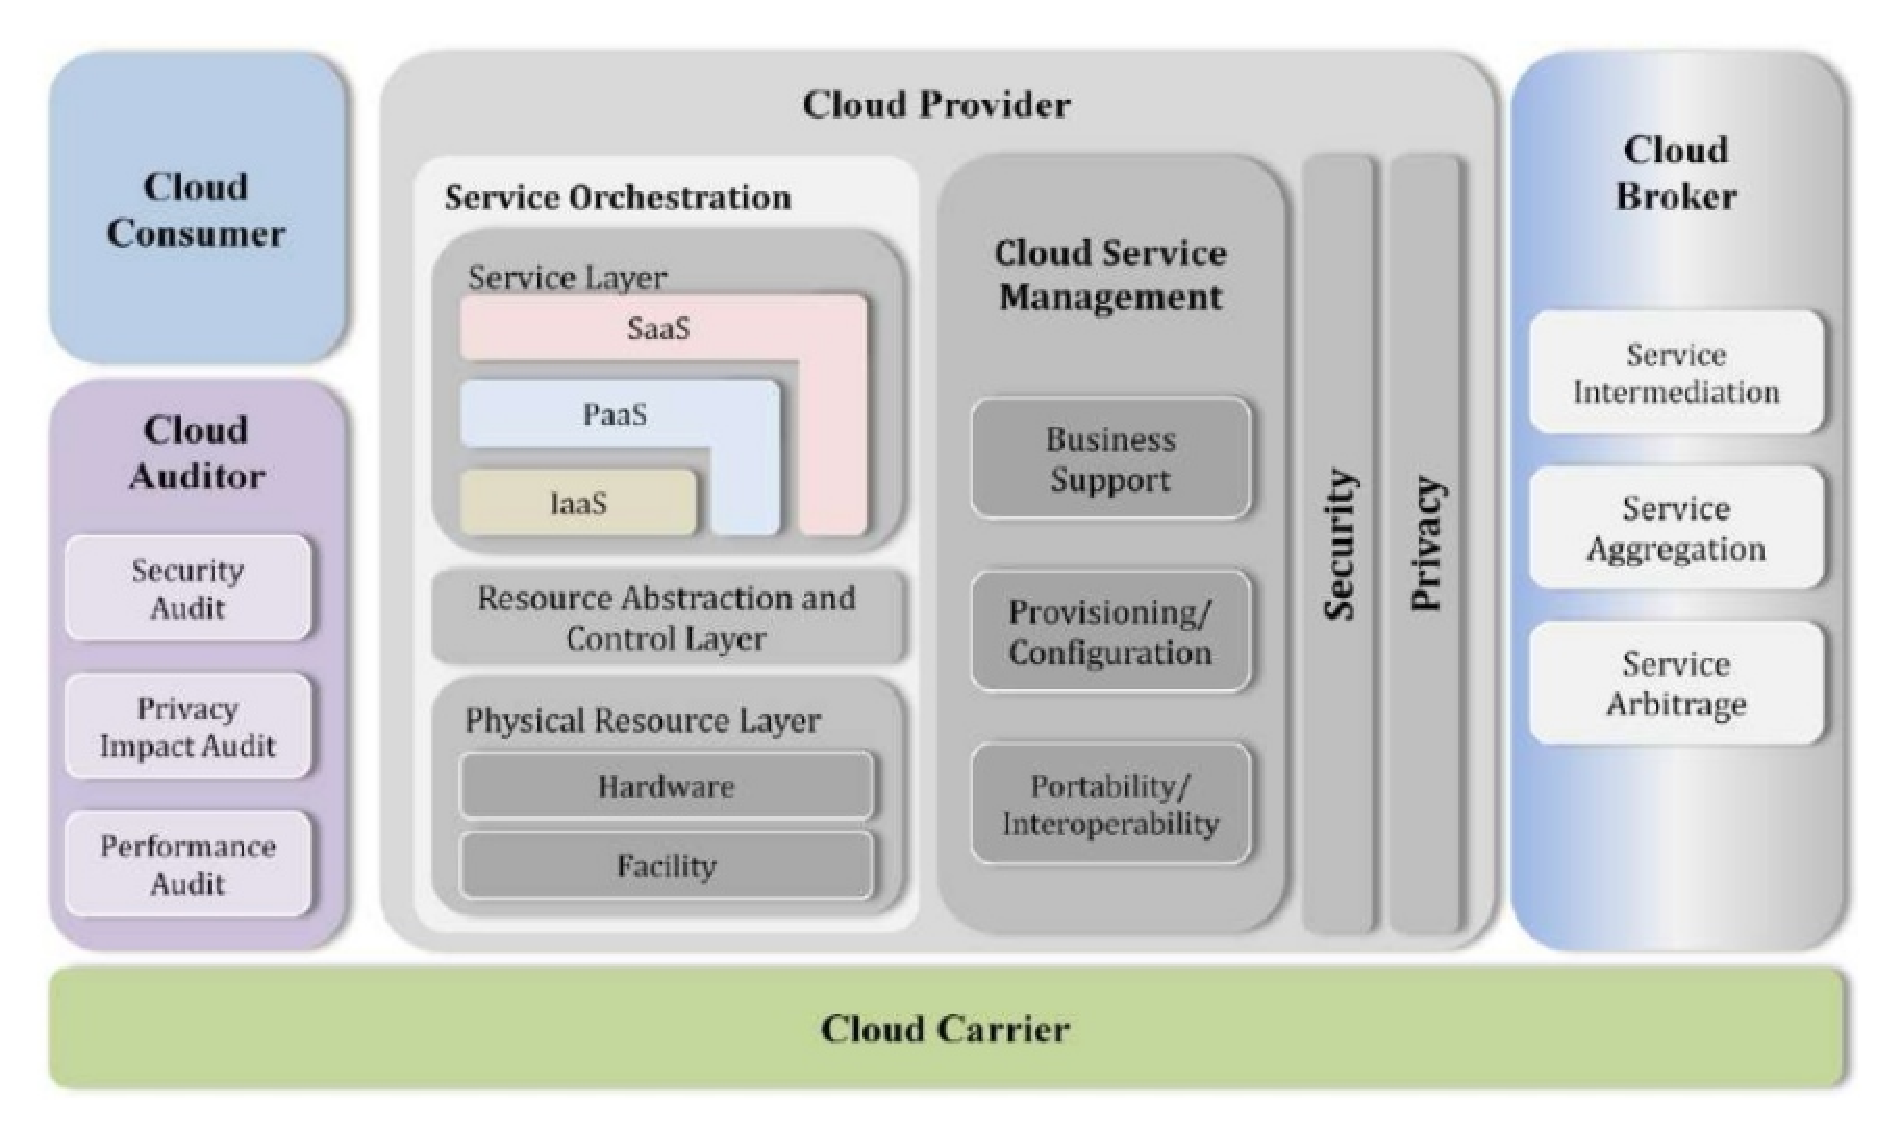
\includegraphics[scale=0.5]{imagens/cloudarch.eps}
  	\caption{Arquitetura de referência para Cloud Computing}
	\end{figure}

	\subsection{Cloud Consumer}
	Representa classes de consumidores para cada modelo possível de serviço. 

	No caso de SaaS são diversos departamentos operacionais de uma empresa, consumindo serviços de ERP, CRM, vendas, finanças, RH, redes sociais, webmail etc. 

	No caso de PaaS são os setores de análise de dados e desenvolvimento, que consomem serviços de BI, banco de dados, \textit{deployment} de aplicações, integração de sistemas e desenvolvimento e testes.

	Por fim, os consumidores de IaaS são os setores da empresa responsável pela infraestrutura e IT, que consomem serviços de backup e recuperação, gerenciamento de serviços, armazenamento, hospedagem de plataformas etc.

	\subsection{Cloud Auditor}
	Cloud Auditor é o componente responsável por relatar e registrar as ações relativas a segurança, privacidade e performance da nuvem, tanto para fins de transparência para os consumidores quanto de regulamentação governamental para rastrear atividades suspeitas e irregulares. Pode ser tanto um órgão governamental ou uma entidade fiscalizadora global na Internet.

	\subsection{Cloud Provider}
	Cloud Provider é o provedor de nuvem como a \textit{Amazon Web Services}, \textit{Microsoft Azure}, \textit{Netflix}, \textit{Youtube}, dentre outros. Dependendo das categorias de modelo de serviço em que o provedor se encaixa, ele poderá ter camadas de serviço de SaaS, PaaS ou IaaS. 

	As principais atividades do Cloud Provider são a implantação de serviços, a orquestração de serviços, o gerenciamento de serviços, a segurança e por fim, a privacidade. Deve gerenciar e abstrair toda lógica de controle e a camada física de recursos de hardware, bem como as instalações e locais físicos.

	\subsection{Cloud Broker}
	O Cloud Broker é responsável por uma espécie de serviço de corretagem. Este ator no ecossistema de nuvem é responsável por oferecer serviços de proteção jurídica durante a negociação de contratos com provedores de nuvem. 

	Oferece também serviços de diminuição de custos com o provedor, agregando diversos serviços a fim de obter o melhor custo-benefício.

	Por fim, pode oferecer serviços diferenciados, como um serviço adicional de segurança, para proteger o consumidor de vazamento de dados na nuvem.


	\subsection{Cloud Carrier}
	O Cloud Carrier são todas entidades responsáveis por disponibilizar a conexão e transporte de serviços na nuvem entre consumidores e provedores (Companhias de redes, telecomunicações, dispositivos de acesso e IoT). 